
\documentclass[10pt,conference]{IEEEtran}
\usepackage{amsmath,amssymb,amsfonts}
\usepackage{graphicx}
\usepackage{booktabs}
\usepackage{url}
\usepackage{xcolor}
\usepackage{cite}
\usepackage{array}
\usepackage{caption}
\usepackage{placeins}
\graphicspath{{../figures/}}

\title{Feasibility-Aware Quantum-Compatible Benchmarking of HUBO/QUBO Formulations for UAV Obstacle-Avoidance and Visibility-Aware Grid Planning}

\author{\IEEEauthorblockN{Author names to be finalized}
\IEEEauthorblockA{Affiliations to be finalized\\
Email: to be finalized}}

\begin{document}
\maketitle

\begin{abstract}
Quantum-assisted UAV path planning has recently been studied using QAOA-style obstacle-avoidance formulations, but a low-energy binary sample is not necessarily a valid UAV trajectory. This paper presents a feasibility-aware benchmark for an $8\times8$, $L=20$ UAV grid-planning problem with obstacle avoidance, line-of-sight visibility cost, and a higher-order temporal buffer-risk term. The model uses binary variables $x_{t,v}$ indicating whether the UAV occupies cell $v$ at time layer $t$ and forms a HUBO objective with one-hot, start, motion, obstacle, visibility, terminal-goal, and sustained near-obstacle proximity terms. The instance has 1,280 original binary variables and 118,344 polynomial terms, including 4,392 cubic monomials. We compare A*, RRT-best, a QUAV-style QAOA candidate-path selector, native trajectory-level simulated annealing (SA), D-Wave Ocean's classical \texttt{neal} sampler after HUBO-to-QUBO reduction, and a new exact CP-SAT/MILP baseline that minimizes the native HUBO soft objective over hard-feasible paths. The uploaded CP-SAT run reports OPTIMAL and certifies that the best observed SA path is globally optimal for the enforced feasible-path objective, with native HUBO energy $-20752.43$, soft cost 247.57, path length 14, six turns, and 85\% visibility. The paper now also shows the decoded optimized paths for all compared methods, making the geometric differences and failure modes visible. The QUAV-style selector produces a valid low-turn geometric path, but it is not optimal under the native HUBO objective. \texttt{neal} obtains nonzero structural feasibility and goal-arrival rates separately but zero full-task success in 50 reads. The results do not claim quantum speedup; they show that feasibility-aware decoding, exact baselines, and quadratization accounting are essential for interpreting quantum-compatible UAV planning results.
\end{abstract}

\begin{IEEEkeywords}
HUBO, QUBO, feasibility-aware benchmarking, UAV path planning, obstacle avoidance, visibility-aware planning, MILP, CP-SAT, QAOA, quantum-compatible optimization.
\end{IEEEkeywords}

\section{Introduction}
UAV path planning in cluttered environments requires at least two safety properties: the path must avoid obstacles, and the decoded plan must be executable under the allowed motion model. When perception or tracking is relevant, the planner may also prefer cells with line of sight to the target. Recent quantum-assisted work such as QUAV formulates UAV obstacle-avoidance path planning using QAOA-style optimization and compares against A* and RRT. QUAV is therefore an important closest reference for quantum-assisted UAV navigation. However, a QAOA, annealing, or QUBO solver returns a binary sample, and the sample must be decoded and checked before it can be called a valid path.

This paper studies a deliberately compact grid abstraction so that modeling and solver behavior can be inspected directly. The goal is not to claim quantum speedup on a small static grid. The goal is to define a reproducible HUBO/QUBO-compatible benchmark, separate energy minimization from actual path validity, and compare classical, quantum-inspired, and quantum-compatible solver pathways on the same problem instance.

The contributions are as follows. First, we give a complete binary decision-variable formulation for UAV grid planning with obstacle avoidance and a visibility cost. Second, we identify the real source of higher-order structure: a temporal buffer-risk term, not the static line-of-sight cost. Third, we introduce a feasibility-aware evaluation protocol that reports structural feasibility, goal arrival, and full-task success separately. Fourth, we implement a same-platform QUAV-style QAOA candidate-path baseline, clearly not as official QUAV code but as a reproducible reference following the published workflow. Fifth, we add an exact CP-SAT baseline and a companion MILP implementation, enabling global comparison against the native HUBO soft objective over hard-feasible paths.

\section{Discrete Planning Model}
Let $G=(V,E)$ be an $N\times N$ grid graph. In the experiments $N=8$, $|V|=64$, and time layers are indexed $t=0,\ldots,L-1$ with $L=20$. Let $O\subset V$ be the obstacle set, $s\in V$ the start cell, and $g\in V$ the target cell. The permitted next-cell set is
\begin{equation}
\mathcal{N}(u)=\{u\}\cup\{v\in V:(u,v)\in E\},
\end{equation}
where the self-loop represents hovering.

The binary state variable is
\begin{equation}
 x_{t,v}\in\{0,1\},\qquad x_{t,v}=1 \Leftrightarrow \text{the UAV is at cell }v\text{ at time }t.
\end{equation}
A valid binary solution decodes to a trajectory $\pi=(v_0,\ldots,v_{L-1})$ only if exactly one state variable is active at every layer.

Let $\mathrm{LOS}(u,g)$ denote the rasterized Bresenham line cells strictly between $u$ and $g$. The per-cell visibility/occlusion-depth surrogate is
\begin{equation}
 C_{\mathrm{occ}}(u)=|\mathrm{LOS}(u,g)\cap O|.
\end{equation}
A zero value indicates clear line of sight in this grid model. Let $B\subset V\setminus O$ be the set of non-obstacle cells within Chebyshev distance one of an obstacle. Cells in $B$ are legal but risky.

\section{HUBO Formulation}
The total polynomial objective is
\begin{equation}
\begin{split}
H(x) = &H_{\mathrm{uniq}} + H_{\mathrm{start}} + H_{\mathrm{move}} + H_{\mathrm{obs}} \\
&+ H_{\mathrm{occ}} + H_{\mathrm{prox}} + H_{\mathrm{goal}} + H_{\mathrm{term}} .
\end{split}
\end{equation}
The structural terms are
\begin{align}
H_{\mathrm{uniq}} &= \lambda_u \sum_{t=0}^{L-1}\left(\sum_{v\in V} x_{t,v}-1\right)^2,\\
H_{\mathrm{start}} &= \lambda_s(1-x_{0,s}),\\
H_{\mathrm{move}} &= \lambda_m\sum_{t=0}^{L-2}\sum_{u\in V}\sum_{v\notin\mathcal{N}(u)}x_{t,u}x_{t+1,v},\\
H_{\mathrm{obs}} &= \lambda_o\sum_{t=0}^{L-1}\sum_{v\in O}x_{t,v}.
\end{align}
The static visibility cost is linear:
\begin{equation}
H_{\mathrm{occ}}=\lambda_{\mathrm{occ}}\sum_{t=0}^{L-1}\sum_{u\in V}C_{\mathrm{occ}}(u)x_{t,u}.
\end{equation}
The sole cubic term is the sustained-proximity penalty:
\begin{equation}
H_{\mathrm{prox}}=\lambda_p \eta \sum_{t=1}^{L-2}\sum_{u\in B}\sum_{v\in B\cap\mathcal{N}(u)}\sum_{w\in B\cap\mathcal{N}(v)}x_{t-1,u}x_{t,v}x_{t+1,w}.
\end{equation}
Here $\eta=3$. This term penalizes remaining in connected buffer cells for three consecutive layers. Thus the model is genuinely HUBO, but the higher-order degree comes from temporal buffer-risk modeling rather than from static visibility.

The goal terms are
\begin{align}
H_{\mathrm{goal}} &= \lambda_g\sum_{t=0}^{L-1}\sum_{v\in V}\frac{t+1}{L}\|p_v-p_g\|_2x_{t,v},\\
H_{\mathrm{term}} &= \lambda_{\mathrm{term}}\sum_{v\ne g}x_{L-1,v}.
\end{align}
The updated instance uses $\lambda_u=\lambda_s=\lambda_m=\lambda_o=1000$, $\lambda_{\mathrm{occ}}=10$, $\lambda_p=5$, $\lambda_g=8$, $\lambda_{\mathrm{term}}=50$, and $\eta=3$.

\section{Feasibility-Aware Evaluation}
A solver output is not scored only by total HUBO energy. Each binary sample is decoded and checked directly. We report: structural feasibility, meaning one-hot occupancy, correct start, legal transitions, and no obstacle occupancy; goal arrival, meaning $v_{L-1}=g$; and full-task success, meaning both conditions hold for the same decoded sample. Soft cost and native HUBO energy are then interpreted on valid decoded paths.

This distinction is essential for QUBO/BQM and QAOA-style workflows. A sample can have a low reduced-model energy while failing one-hot, motion, obstacle, or target-arrival checks. Such a sample is not a UAV plan. The benchmark therefore reports feasibility rates and representative decoded trajectories, not energy alone.

\section{Solvers and Implementation}
\subsection{A* and RRT Baselines}
A* searches directly on the grid with obstacle avoidance and a heuristic path cost. RRT-best is a randomized grid planner used as a sampling-style reference. These methods return explicit paths and are checked with the same feasibility evaluator.

\subsection{QUAV-Style QAOA Baseline}
QUAV maps UAV path segments to qubits and applies QAOA-style optimization with obstacle-buffer costs. Since no official public code was available in this workflow, we implemented a QUAV-style candidate-path selector following the published algorithmic description. It generates collision-free candidate paths, assigns a QUAV-style geometric cost using length, buffer steps, and turns, and uses a small QAOA-style one-hot selector over the candidates. This baseline is a same-platform reference only, not an exact reproduction of the authors' implementation.

\subsection{Trajectory-Level SA and \texttt{neal}}
Trajectory-level SA searches over cell sequences and evaluates the native HUBO energy directly, including the cubic term. Its proposal operator preserves one-hot occupancy, start, legal motion, and obstacle avoidance by construction. In contrast, D-Wave Ocean's \texttt{neal} is a classical BQM sampler. Therefore the HUBO is first reduced to a QUBO/BQM with auxiliary variables and quadratization penalties before sampling.

\subsection{Exact MILP and CP-SAT Baselines}
We added exact optimization baselines in both CP-SAT and MILP form. Both encodings enforce the path constraints directly: exactly one cell per layer, fixed start, final target arrival, obstacle cells forbidden, and legal transitions. Auxiliary binary variables linearize each cubic proximity monomial $y_{tuvw}=x_{t-1,u}x_{t,v}x_{t+1,w}$. The objective minimizes
\begin{equation}
H_{\mathrm{occ}}+H_{\mathrm{prox}}+H_{\mathrm{goal}}+H_{\mathrm{term}}
\end{equation}
over the hard-feasible set. Because all hard constraints are enforced, every feasible solution has the same hard contribution $-\lambda_u L-\lambda_s=-21000$ under the expanded HUBO implementation. The native HUBO energy is therefore this hard constant plus the optimized soft cost. The CP-SAT model uses OR-Tools and the MILP model uses a linear mixed-integer encoding. The uploaded CP-SAT run returned OPTIMAL, so its solution is used as the exact baseline in the final table.

\section{Results}
Table~\ref{tab:instance} summarizes the updated instance.
\begin{table}[t]
\caption{Updated main HUBO instance.}
\label{tab:instance}
\centering
\begin{tabular}{lr}
\toprule
Quantity & Value\\
\midrule
Grid size & $8\times 8$\\
Horizon $L$ & 20\\
Original binary variables & 1,280\\
Total polynomial terms & 118,344\\
Linear terms & 1,280\\
Quadratic terms & 112,672\\
Cubic terms & 4,392\\
Obstacles & 6\\
Buffer cells & 24\\
\bottomrule
\end{tabular}
\end{table}





\begin{table}[t]
\centering
\scriptsize
\caption{Unified same-platform comparison. For deterministic or single-output methods, feasibility columns indicate whether the returned path satisfies the condition. For stochastic solvers, feasibility columns report empirical rates over 50 runs/reads.}
\label{tab:unified}
\resizebox{\columnwidth}{!}{%
\begin{tabular}{lccccccccc}
\toprule
Method & Feas. & Goal & Full & Len. & Turns & Buf. & Vis. & HUBO E & Time\\
\midrule
A* & Yes & Yes & Yes & 14 & 7 & 4 & 85.0\% & -20742.26 & 0.028s\\
RRT & Yes & Yes & Yes & 14 & 5 & 4 & 70.0\% & -20700.19 & N/R\\
QUAV-QAOA & Yes & Yes & Yes & 14 & 1 & 3 & 80.0\% & -20725.94 & 4.11s\\
CP-SAT exact & Yes & Yes & Yes & 14 & 6 & 4 & 85.0\% & -20752.43 & 1.02s\\
HUBO-SA & 100.0\% & 16.0\% & 16.0\% & 14 & 6 & 4 & 85.0\% & -20752.43 & 1207.26s\\
QUBO/\texttt{neal} & 12.0\% & 8.0\% & 0.0\% & 18 & 12 & 2 & 20.0\% & -20060.47 & 6.15s\\
\bottomrule
\end{tabular}%
}
\end{table}


\subsection{Decoded Optimized Paths}
Fig.~\ref{fig:decoded_paths} shows the actual decoded paths returned by each method on the same map. This figure is important because the numerical table alone does not reveal how the methods use the obstacle-buffer region or why different objectives prefer different routes. A*, RRT-best, QUAV-style QAOA, CP-SAT, and the best full-success SA trajectory all reach the target without collisions. The \texttt{neal} panel shows the best-energy decoded QUBO sample; it is structurally feasible but fails to reach the target, explaining why its full-task success rate is zero.

\begin{figure*}[t]
\centering
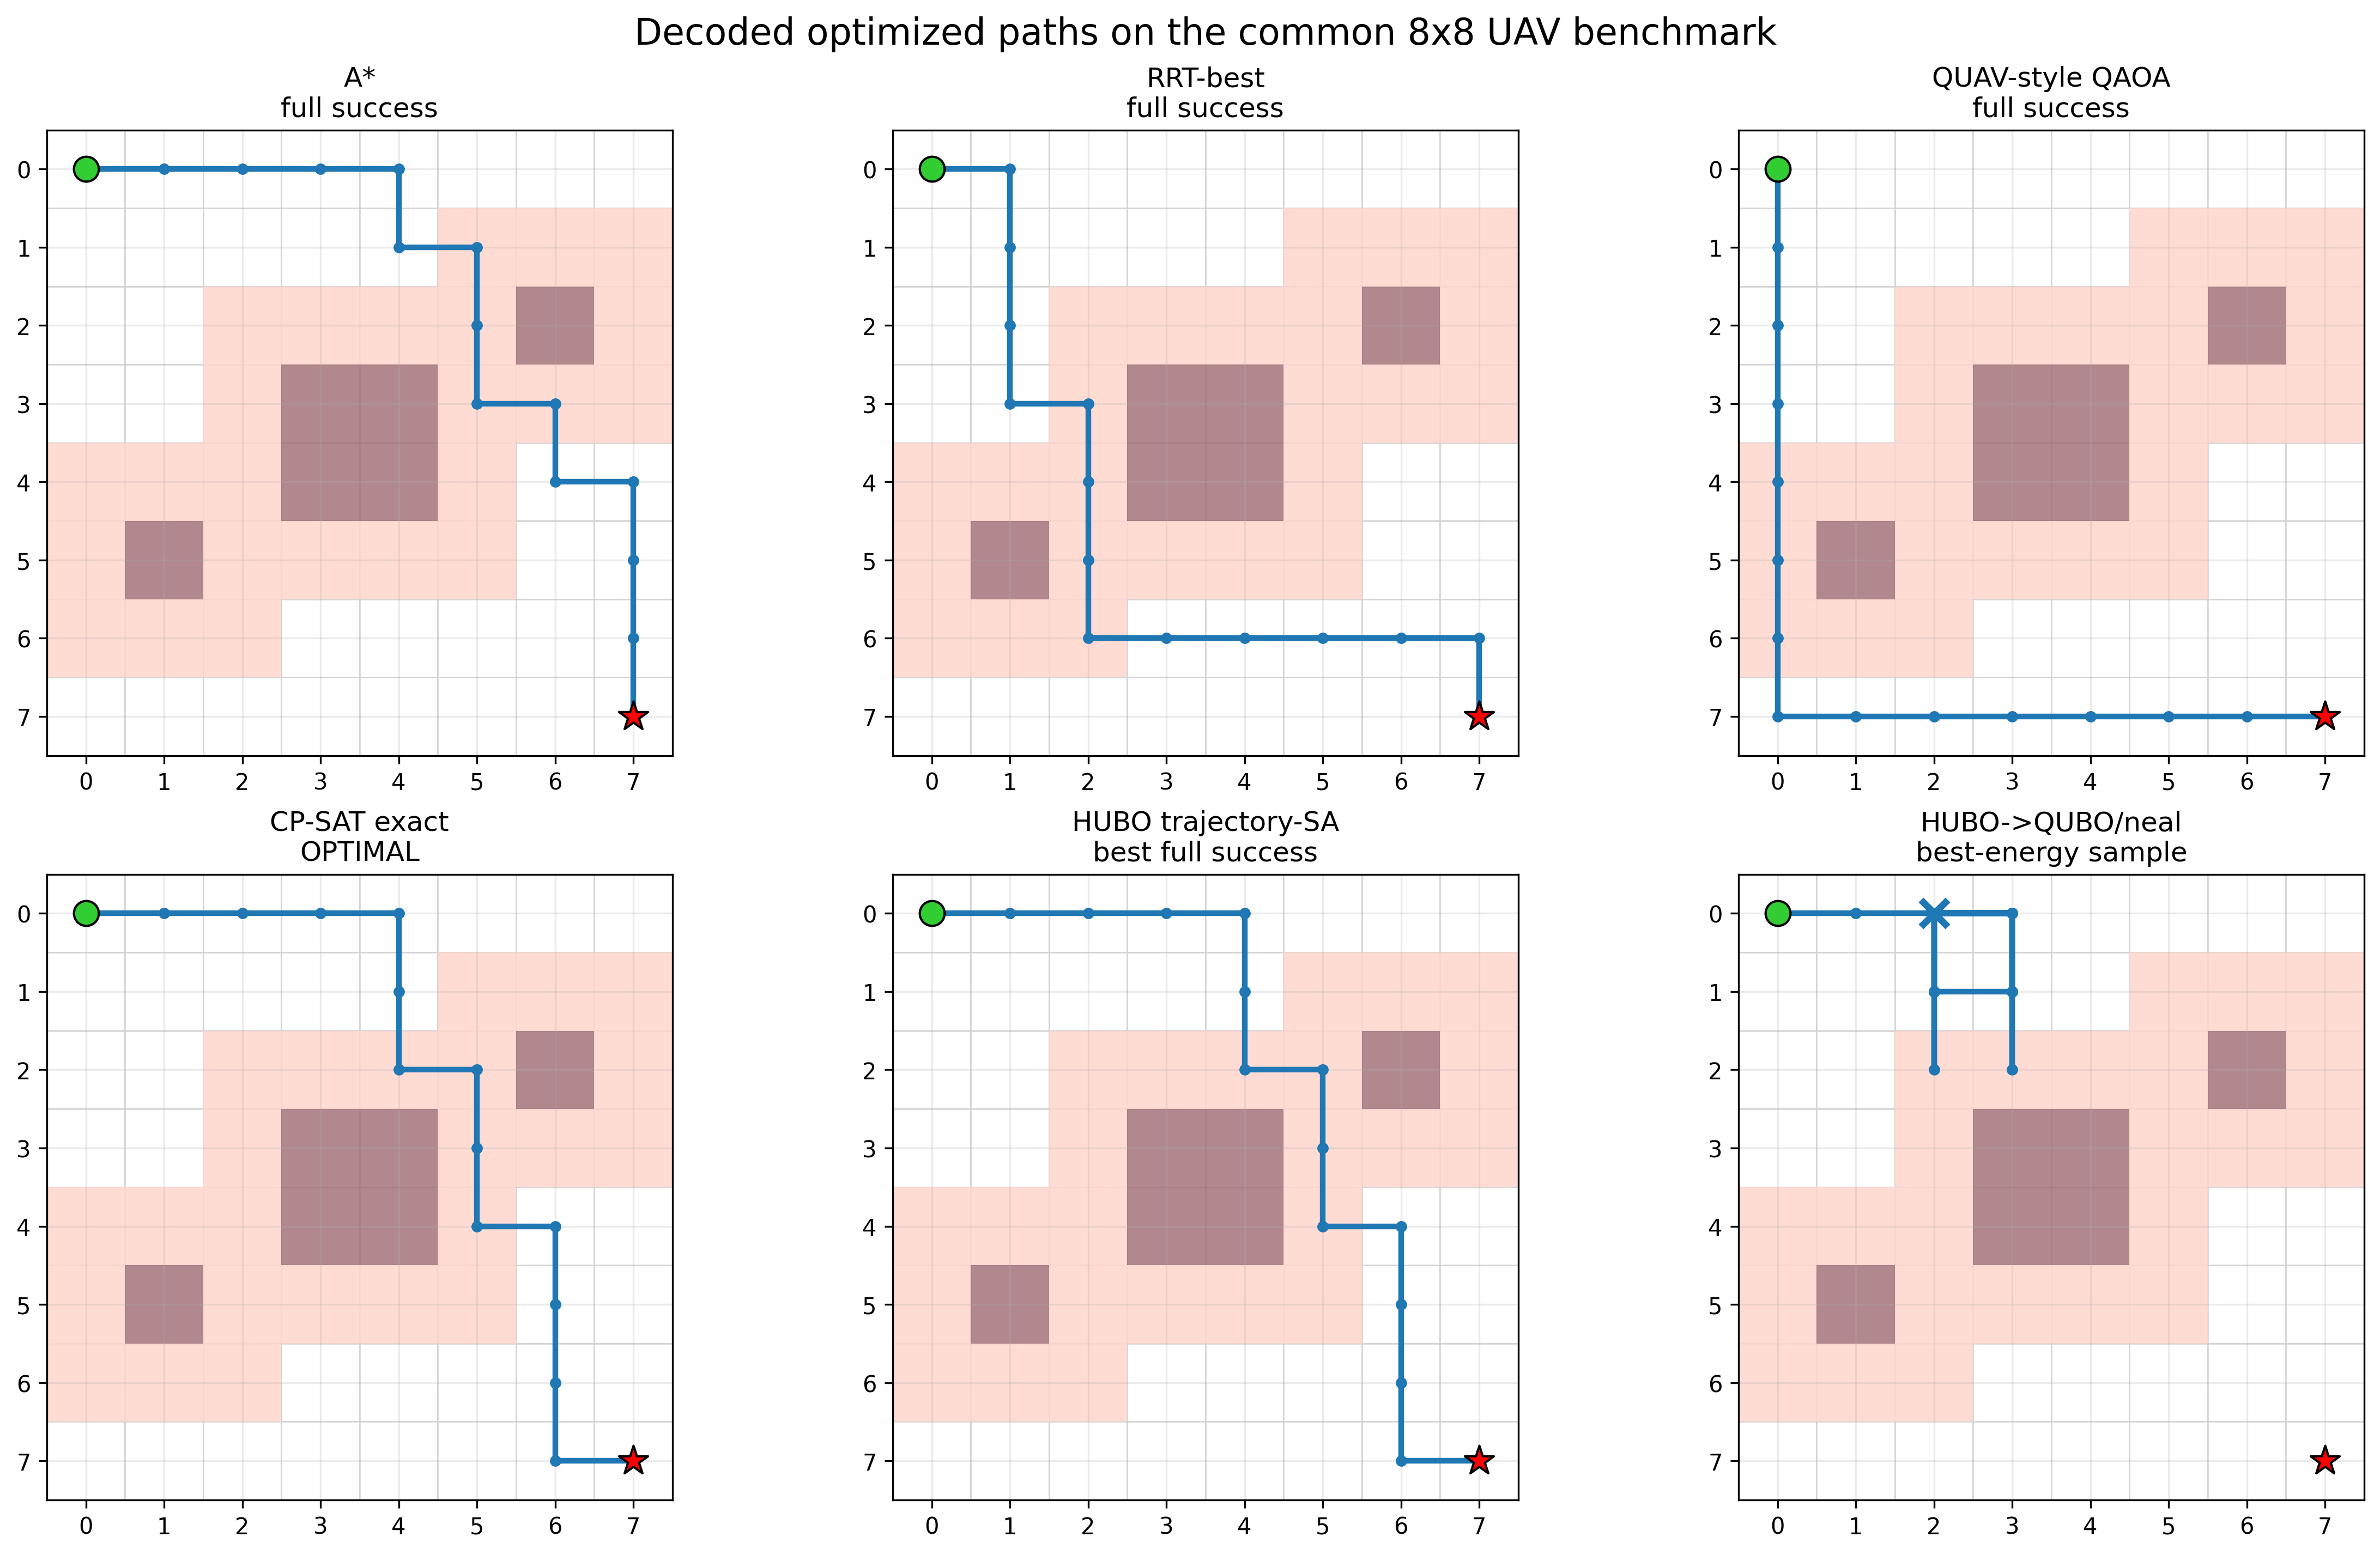
\includegraphics[width=0.98\textwidth]{fig_decoded_paths_all_methods.png}
\caption{Decoded optimized paths on the common $8\times8$, $L=20$ benchmark. Dark cells are obstacles, light cells are obstacle-buffer cells, the green circle is the start, and the red star is the target. The CP-SAT path is globally optimal for the hard-feasible native-HUBO soft objective. The \texttt{neal} path is the best-energy decoded QUBO sample and illustrates a quadratization/sampling failure mode: it is structurally feasible but does not reach the target.}
\label{fig:decoded_paths}
\end{figure*}

The exact CP-SAT baseline reports OPTIMAL, with soft cost 247.57 and native HUBO energy $-20752.43$ in 1.02 s. This matches the best trajectory-SA energy, showing that SA found a globally optimal path for the hard-feasible exact objective on this instance, but SA required 1207.26 s over 50 runs and reached the target in only 8 of 50 runs. A* is much faster and fully successful, but its native HUBO energy is slightly worse because it optimizes a graph-search surrogate rather than the exact cubic proximity-aware objective.

The QUAV-style QAOA selector produces a valid shortest path with only one turn and the lowest QUAV-style geometric cost among its candidates. However, under the native HUBO objective its energy is $-20725.94$, worse than the CP-SAT/SA optimum. This illustrates a central point: a QUAV-style geometric objective and the native HUBO objective are not the same, even when both return collision-free paths. \texttt{neal} after quadratization remains the weakest method in this run: it has 6/50 structural feasibility and 4/50 goal arrival, but 0/50 full-task success.

\begin{figure}[t]
\centering
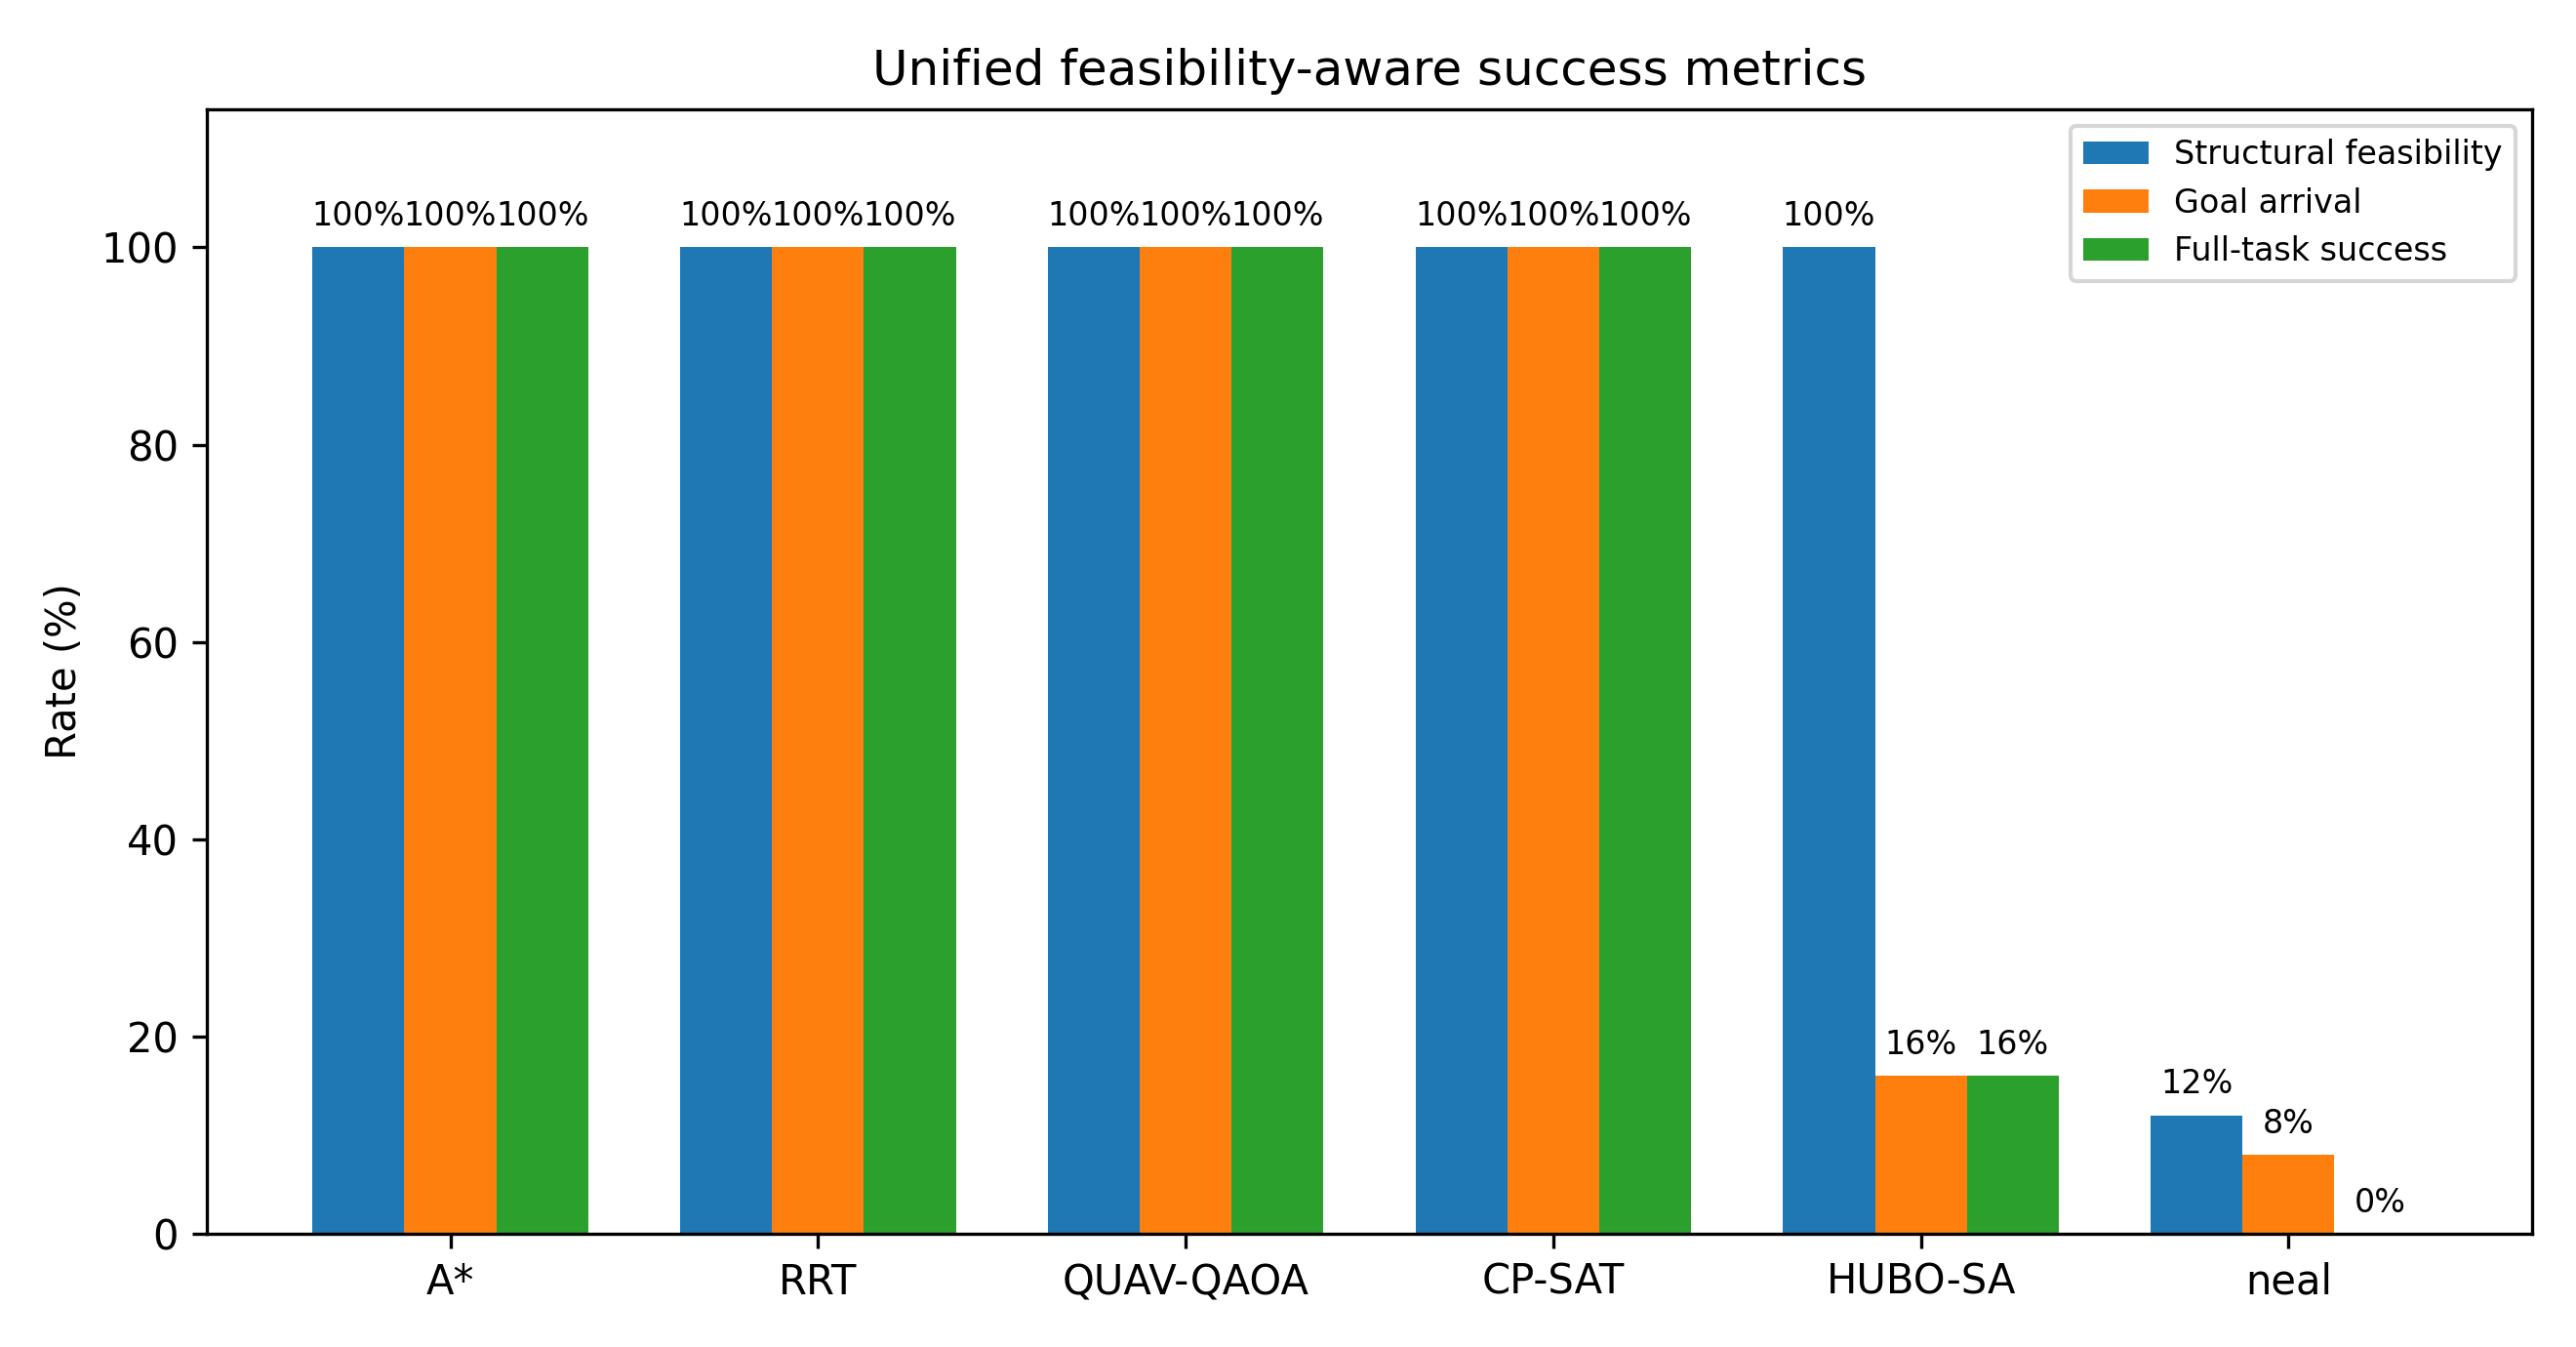
\includegraphics[width=0.98\linewidth]{fig_unified_success_with_cpsat.png}
\caption{Unified feasibility-aware success metrics. The exact CP-SAT run certifies a full-success optimum. \texttt{neal} has nonzero feasibility and goal-arrival rates separately, but zero full-task success.}
\label{fig:unified_success}
\end{figure}


\subsection{Penalty Sweep and QAOA Compatibility}
The penalty-weight sweep for \texttt{neal} shows that weak structural penalties permit low-energy but infeasible samples. In the updated run, structural feasibility was $0/15$ for $\lambda\in\{50,100,300,600\}$, $4/15$ at $\lambda=1000$, and $5/15$ at $\lambda=2000$. The best feasible soft cost improved from 915.4 to 590.6 between $\lambda=1000$ and $\lambda=2000$, still worse than A*, SA, and CP-SAT. A revised $2\times2$, $L=3$ Qiskit QAOA test is included only as a QUBO software-compatibility check, not as a full-instance solver.

\FloatBarrier
\section{Discussion}
The results show why the paper's contribution is not a simple claim that quantum computing outperforms classical planning. On this instance, exact CP-SAT proves the optimum of the hard-feasible native-HUBO soft objective, A* is very fast, and trajectory-SA can find the exact optimum but with poor target-arrival reliability. The decoded paths in Fig.~\ref{fig:decoded_paths} make the solver differences explicit. The QUAV-style QAOA baseline is useful because it shows that a quantum-assisted geometric selector can produce a valid obstacle-free path on the same platform. However, the native HUBO objective distinguishes visibility, temporal buffer-risk, and terminal behavior in a different way. Therefore, same-platform decoded-path evaluation is necessary for fair comparison.

The exact CP-SAT/MILP formulation also clarifies the role of quantum-compatible solvers. If a QUBO sampler is used, it must overcome not only path planning but also one-hot, movement, obstacle, target, and quadratization constraints. The benchmark exposes these failure modes by reporting structural feasibility, goal arrival, and full-task success separately.

\section{Limitations and Future Work}
The model remains a grid abstraction without quadrotor dynamics, velocity, acceleration, heading, camera field-of-view dynamics, or continuous controls. The target is static, so the visibility term is linear; a moving-target formulation would require a separate derivation. The QUAV-style baseline is not official QUAV code. QAOA is currently a small compatibility check rather than a scalable performance result. D-Wave QPU/hybrid execution and larger maps are natural future work. ROS/Gazebo implementation is not required for the present paper because the focus is the optimization and benchmark layer.

\section{Conclusion}
This paper presents a feasibility-aware HUBO/QUBO benchmark and solver-analysis framework for UAV obstacle-avoidance and visibility-aware grid planning. The higher-order structure comes from sustained temporal proximity to obstacle-buffer cells. The unified comparison with A*, RRT-best, QUAV-style QAOA, trajectory-SA, \texttt{neal}, and exact CP-SAT shows that geometric path quality, native HUBO energy, and full trajectory validity are different metrics. The CP-SAT run certifies the best observed SA path as optimal for the hard-feasible native-HUBO soft objective, while \texttt{neal} after quadratization has zero full-task success in the tested reads. The main contribution is therefore a rigorous quantum-compatible benchmark and feasibility-aware evaluation protocol, not a quantum-speedup claim.

\section*{Code Availability}
The code package for this revision includes the HUBO builder, A* baseline, RRT/QUAV-style baseline, trajectory-SA, \texttt{neal} benchmark, exact CP-SAT baseline, companion MILP model, tiny QAOA compatibility check, plotting scripts, and result logs. A public repository or supplementary-material link should be inserted before submission.

\begin{thebibliography}{99}
\bibitem{innan2025quav} N. Innan, M. Kashif, A. Marchisio, Y.-S. Gan, F. Barbaresco, and M. Shafique, ``QUAV: Quantum-assisted path planning and optimization for UAV navigation with obstacle avoidance,'' arXiv:2508.21361, 2025.
\bibitem{hart1968} P. E. Hart, N. J. Nilsson, and B. Raphael, ``A formal basis for the heuristic determination of minimum cost paths,'' \emph{IEEE Trans. Systems Science and Cybernetics}, vol. 4, no. 2, pp. 100--107, 1968.
\bibitem{lavalle1998} S. M. LaValle, ``Rapidly-exploring random trees: A new tool for path planning,'' Tech. Rep. 9811, Iowa State University, 1998.
\bibitem{rosenberg1975} I. G. Rosenberg, ``Reduction of bivalent maximization to the quadratic case,'' \emph{Cahiers du Centre d'Etudes de Recherche Operationnelle}, vol. 17, pp. 71--74, 1975.
\bibitem{glover2019} F. Glover, G. Kochenberger, and Y. Du, ``Quantum bridge analytics I: A tutorial on formulating and using QUBO models,'' \emph{4OR}, vol. 17, pp. 335--371, 2019.
\bibitem{farhi2014} E. Farhi, J. Goldstone, and S. Gutmann, ``A quantum approximate optimization algorithm,'' arXiv:1411.4028, 2014.
\bibitem{dwave_neal} D-Wave Systems, ``dwave-neal simulated annealing sampler,'' software package.
\bibitem{dimod} D-Wave Systems, ``dimod: A shared API for binary quadratic models,'' software package.
\bibitem{qiskit} Qiskit contributors, ``Qiskit, Qiskit Optimization, Qiskit Algorithms, and Qiskit Aer,'' software packages.
\bibitem{scipy} P. Virtanen et al., ``SciPy 1.0: Fundamental algorithms for scientific computing in Python,'' \emph{Nature Methods}, vol. 17, pp. 261--272, 2020.
\bibitem{ortools} L. Perron and V. Furnon, ``OR-Tools,'' Google, software package.
\end{thebibliography}

\end{document}
